\documentclass[xcolor=dvipsnames]{beamer}
\mode<presentation>

\setbeamertemplate{itemize item}[ball]
%\usetheme[secheader]{Boadilla}
%\usetheme{boxes}
\usetheme{myBoadilla}
%\usetheme[secheader]{myBoadilla}
%\usetheme[left]{Goettingen}

%\usepackage{CSIC2}
\setbeamertemplate{itemize item}[ball]
 \setbeamertemplate{navigation symbols}{
      \insertslidenavigationsymbol
%%      \insertdocnavigationsymbol 
%%    {\footnotesize \insertframenumber} %% FIXME: delete if we use CSIC2
 }

\usepackage[absolute,overlay]{textpos}
\usepackage[english]{babel}
\usepackage[latin1]{inputenc}
\usepackage{times}
\usepackage[T1]{fontenc}
% Or whatever. Note that the encoding and the font should match. If T1
% does not look nice, try deleting the line with the fontenc.
%%\usepackage{fancybox}
\usepackage[lined]{algorithm2e}

\usepackage{url}
\newcommand{\cyan}[1]{{\textcolor {cyan} {#1}}}
\newcommand{\blu}[1]{{\textcolor {blue} {#1}}}
\newcommand{\Burl}[1]{\blu{\url{#1}}}
\newcommand{\red}[1]{{\textcolor {red} {#1}}}
\newcommand{\green}[1]{{\textcolor {green} {#1}}}
\newcommand{\mg}[1]{{\textcolor {magenta} {#1}}}
\newcommand{\og}[1]{{\textcolor {PineGreen} {#1}}}
\newcommand{\code}[1]{\texttt{\slshape\footnotesize #1}}
\newcommand{\myverb}[1]{{\footnotesize\texttt {\textbf{#1}}}}
\newcommand{\Rnl}{\ +\qquad\ }
\newcommand{\Emph}[1]{\emph{\mg{#1}}}
\newcommand{\gry}[1]{{\textcolor {gray} {#1}}}

\newcommand{\hanging}[1]{ 
\renewcommand{\baselinestretch}{0.7}\small\normalsize
\setlength{\parskip}{1.5ex plus0ex minus0ex}
  \noindent\hangindent=24pt
  \hangafter=1 
   {\scriptsize #1}
  %\hangindent\parindent
}   


\newcommand{\hango}[1]{ 
\renewcommand{\baselinestretch}{0.7}\small\normalsize
\setlength{\parskip}{1.5ex plus0ex minus0ex}
  \noindent\hangindent=24pt
  \hangafter=1 
   {\tiny #1}
  %\hangindent\parindent
}   


\newcommand{\hanginp}[2]{ 
  \renewcommand{\baselinestretch}{0.7}\small\normalsize
  \setlength{\parskip}{1.5ex plus0ex minus0ex}
  \noindent\hangindent=24pt
  \hangafter=1 
  {\scriptsize #1}{\hspace{2pt}\Large\red{#2}}
  % \hangindent\parindent
}   


%% use for itemize wihtin description
% \newenvironment{myitemize} {
%   \setlength{\leftmarginii}{-10mm}
%   \itemize
% }

% \newenvironment{myitemize}
% {\setlength{\leftmarginii}{-10mm}
% \begin{itemize}}
% {\end{itemize}}


\newenvironment{myitemize}
{\begin{itemize}}{\end{itemize}}


\newcommand{\mydes}[2][]{
  \vspace*{-1pt}
%%  \renewcommand{\baselinestretch}{0.7}\small\normalsize
  \begin{description}\item[{#2}]{#1}\end{description}
\vspace*{-8pt}
}


\usepackage{gitinfo}


\title{BM-1: a 9 minute intro}



\author[R. Diaz-Uriarte]{Ram�n Diaz-Uriarte} %% \\ \Burl{http://ligarto.org/rdiaz}}

\institute[]{Department of Biochemistry\\
Universidad Aut�noma de Madrid\\
Madrid, Spain\\
\texttt{ramon.diaz@iib.uam.es}\\
\Burl{http://ligarto.org/rdiaz}
}


% \date[22-09-2014]{22-September-2014}
% \date{\gitAuthorDate\ {\footnotesize (Rev: \gitAbbrevHash)}}
\date[15-09-2014]{15-September-2014\\ {\tiny (Rev: \gitAbbrevHash)}}


\begin{document}


\begin{frame}
  \titlepage
\end{frame}


% \begin{frame}
%    \frametitle{Outline}
%  {\small
%  \tableofcontents[subsectionstyle=hide]
%  }
%  \end{frame}



\begin{frame}
  \frametitle{Organization and long presentation of BM-1}
  \begin{itemize}
  \item Monday, 22-September-2014, 10:00 (am, of course!), Aula Magna
  \end{itemize}
\end{frame}



\begin{frame}
  \frametitle{Your homework for tomorrow}
  \begin{itemize}
  \item Make sure you can access Moodle:
    \Burl{http://ciencias.biomol.uam.es/moodle}
\vspace*{15pt}
  \item This is \textbf{NOT} the usual UAM moodle (i.e., \textbf{this is not} \Burl{http://moodle.uam.es}).
  \end{itemize}
\end{frame}



\begin{frame}
  \frametitle{What Moodle will look like}
\vspace*{10pt}
   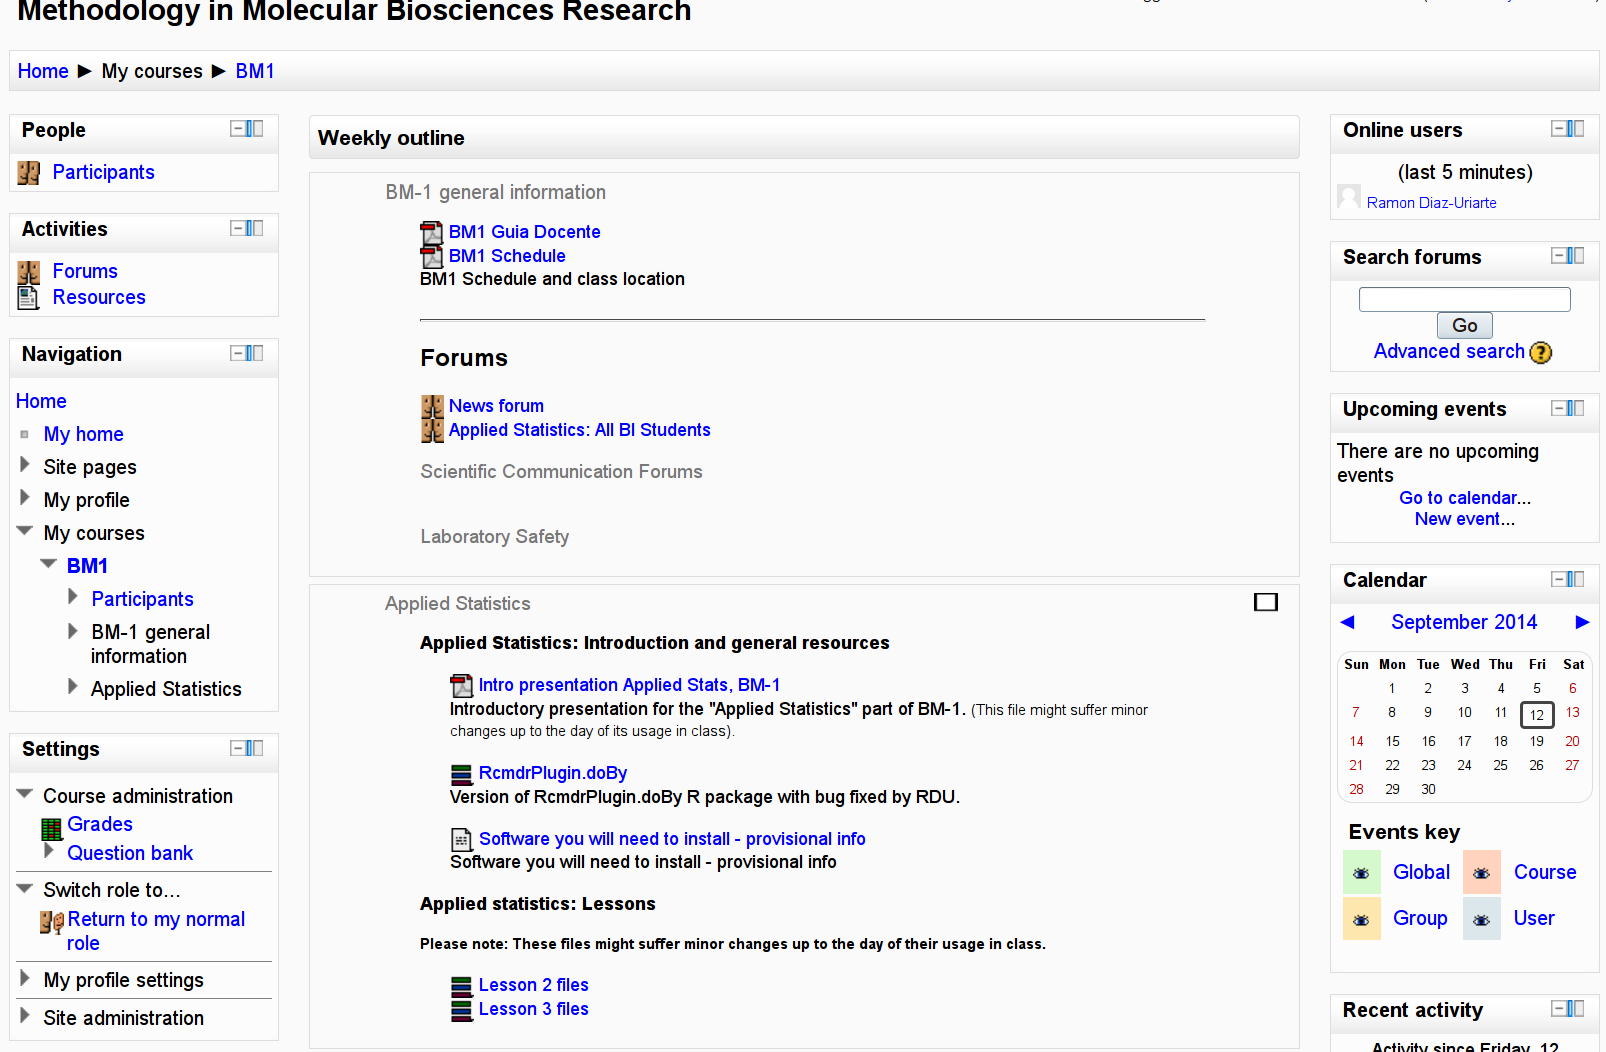
\includegraphics[%
   width=12.5cm,
   keepaspectratio]{moodle-view.png}
\end{frame}





\begin{frame}
  \frametitle{Your homework for tomorrow}
  \begin{itemize}
  \item You should have received an email about BM-1.
  \item If problems with Moodle, come tomorrow Tuesday 16 to Seminarios 4
    and 5, from 10:00 to 13:00 (better if you are there at 10:00).
  \end{itemize}
\end{frame}



\begin{frame}
  \frametitle{Other homework (ASAP)}
  \begin{enumerate}
  \item Get your UAM email: all issues to CAU (google for ``UAM cau email'').
  \item {\scriptsize (If you plan on using your computer around campus)} Enable Wifi
    access (google for ``UAM wifi'').
  \end{enumerate}
\end{frame}


\begin{frame}
  \frametitle{Software for BM-1}
  \begin{itemize}
  \item An updated list available by 19-September.
  \end{itemize}
\end{frame}



\begin{frame}
  \frametitle{Schedule}
  \begin{itemize}
  \item Available from Moodle.
  \end{itemize}
\end{frame}



\begin{frame}
  \frametitle{How the schedule looks like}
\vspace*{10pt}
   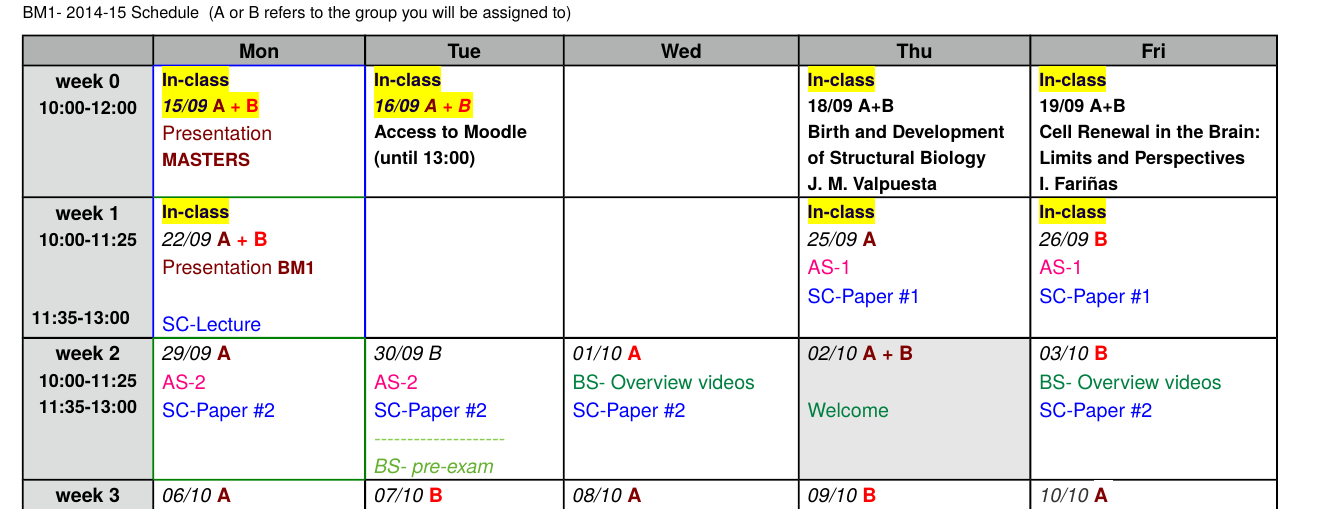
\includegraphics[%
   width=12.5cm,
   keepaspectratio]{schedule-view.png}
\end{frame}



\begin{frame}
  \frametitle{Schedule: key dates}
Key dates until 22-September:
    \begin{description}
    \item[Access to Moodle] 16-September, Seminarios 4 y 5. 10:00--13:00.
    \item[J.\ M.\ Valpuesta's talk] 18-September. Aula Magna. 10:00--12:00.
    \item[I.\ Fari�a's talk] 19-September. Aula Magna. 10:00--12:00.
    \item[Presentation and first class BM-1] 22-September. Aula Magna. 10:00--13:00. 
    \end{description}
\end{frame}



\begin{frame}
  \frametitle{A copy of this PDF?}
\Burl{http://ligarto.org/rdiaz/First-day-BM1.pdf}
\end{frame}


\end{document}

